\section{Simplex}
Das Simplex ist ein Begriff, welcher aus der Geometrie stammt. Es beschreibt ein n-dimensionales Polytop. Wobei ein Polytop die Bezeichnung f"ur ein verallgemeinertes Polygon ist, sprich ein verallgemeinertes Vieleck. 
Hier einige vorstellbare Beispiele zum Simplex:
 
\begin{tabular}{c|l}
Dimension & Geometrische Form\\
\hline
$n=0$ & Punkt\\
$n=1$ & Strecke\\
$n=2$ & Dreieck\\
$n=3$ & Tetraeder
\end{tabular}

\begin{figure}
\centering
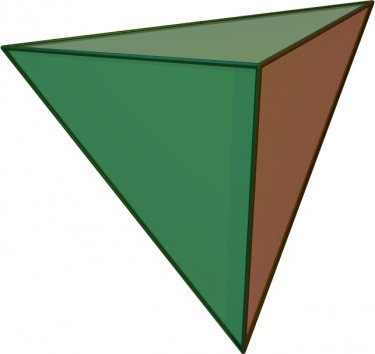
\includegraphics[height=0.25\textwidth]{../bilder/tetraeder.jpg}
\caption{Tetraeder als Beispiel eines Simplex für $n=3$}
\end{figure}

Aus der Tabelle wird ersichtlich, dass jedes $n$-dimensionale Simplex genau $n+1$ Ecken hat.
Im Downhill-Simplex-Verfahren wird das Simplex ben"otigt, um die optimalen Parameterwerte zu finden. Man kann es sich so vorstellen, dass das Simplex im n-dimensionalen Parameterraum aufgespannt wird und dann f"ur jeden seiner Eckpunkte den entsprechenden Funktionswert (auf Grund der Zielfunktion) berechnet. \\
Wie in der Einleitung schon erw"ahnt worden ist, arbeitet der Simplex-Downhill Algorithmus ohne Ableitungen. Warum das funktioniert wird klar, wenn man sich vorstellt, dass das Simplex selber auf der Zielfunktion liegt und sozusagen die Ableitung imitiert. Sucht der Algorithmus ein Minimum, so bewegt er sich nat"urlich abw"arts (downhill), was auch seine Namensgebung erkl"art. Der Algorithmus ist aber ebenfalls in der Lage nach Maxima zu suchen, wobei im Folgenden nur die Suche nach Minima behandelt wird.\\
Hat man das Simplex auf der Zielfunktion platziert, werden die berechneten Testpunkte gepr"uft, wobei der schlechteste dieser Punkte dann mittels gewisser "Taktiken" ersetzt wird. Dies wird solange fort gef"uhrt, bis das gew"unschte Ergebnis erreicht worden ist.\\ 
Im n"achsten Abschnitt werden die m"oglichen Taktiken, um das Simplex zu ver"andern, genauer erl"autert. 

%--------------------------------------------------------------------------------------------------------------------------------------------

\section{Modifikationen des Simplex}
Die M"oglichkeiten das Simplex soweit zu ver"andern, dass es den optimalen Punkt findet, sind begrenzt.
Die Darstellungen beziehen sich hierbei auf einen Simplex der zweiten Dimension (Dreieck), nat"urlich gelten diese Modifikationen auch f"ur einen n-dimensionalen Simplex. Der Algorithmus w"ahlt auf Grund der Werte der Eckpunkte beziehungsweise deren Zielfunktionswerte die Modifikationsart aus (siehe Kapitel XXX).

\begin{figure}[h]
	\centering
	\definecolor{uuuuuu}{rgb}{0.27,0.27,0.27}
\definecolor{zzttqq}{rgb}{0.6,0.2,0}
\definecolor{qqqqff}{rgb}{0,0,1}
\begin{tikzpicture}[line cap=round,line join=round,>=triangle 45,x=1.0cm,y=1.0cm]
\clip(5.32,0.26) rectangle (11.46,4.08);
\fill[color=zzttqq,fill=zzttqq,fill opacity=0.1] (5.74,2.92) -- (10.36,3.74) -- (11,1.52) -- cycle;
\draw [color=zzttqq] (5.74,2.92)-- (10.36,3.74);
\draw [color=zzttqq] (10.36,3.74)-- (11,1.52);
\draw [color=zzttqq] (11,1.52)-- (5.74,2.92);
\draw [color=zzttqq] (11,1.52)-- (5.74,2.92);
\begin{scriptsize}
\fill [color=qqqqff] (5.74,2.92) circle (1.5pt);
\draw[color=qqqqff] (5.75,3.02) node {$x_{min}$};
\fill [color=qqqqff] (10.36,3.74) circle (1.5pt);
\draw[color=qqqqff] (10.51,3.81) node {$x_{max}$};
\fill [color=qqqqff] (11,1.52) circle (1.5pt);
\draw[color=qqqqff] (11.07,1.59) node {$x_3$};
\fill [color=uuuuuu] (9.03,2.73) circle (1.5pt);
\draw[color=uuuuuu] (9.13,2.7) node {$x_m$};
\end{scriptsize}
\end{tikzpicture}
%
  	\caption{Simplex im zweidimensionalen Raum}%
	\label{fig:Dreieck}%
\end{figure}

\subsection{Reflexion}
Bei der Reflexion wird der schlechteste Punkt $x_{max}$ am Schwerpunkt des Simplex gespiegelt und mit einem Faktor $\alpha$ gewichtet: 
\begin{equation}
x_{ref} = x_m + \alpha \cdot (x_m-x_{max})
\end{equation}
Wenn ein neues Simplex berechnet werden muss, weil der optimale wert noch nicht gefunden worden ist, dann wird die Reflexion IMMER durchgef"uhrt, daher wird in den folgenden Methoden manchmal mit $x_{ref}$ anstatt mit $x_{max}$ gerechnet. Wenn man den Algorithmus unter XXX betrachtet, erkennt man, warum das so ist.  
\begin{figure}[h]
	\centering
	\definecolor{uuuuuu}{rgb}{0.27,0.27,0.27}
\definecolor{zzttqq}{rgb}{0.6,0.2,0}
\definecolor{qqqqff}{rgb}{0,0,1}
\begin{tikzpicture}[line cap=round,line join=round,>=triangle 45,x=1.0cm,y=1.0cm]
\clip(5.32,0.26) rectangle (11.46,4.08);
\fill[color=zzttqq,fill=zzttqq,fill opacity=0.1] (5.74,2.92) -- (10.36,3.74) -- (11,1.52) -- cycle;
\fill[color=zzttqq,fill=zzttqq,fill opacity=0.1] (5.74,2.92) -- (7.71,1.71) -- (11,1.52) -- cycle;
\draw [color=zzttqq] (5.74,2.92)-- (10.36,3.74);
\draw [color=zzttqq] (10.36,3.74)-- (11,1.52);
\draw [color=zzttqq] (11,1.52)-- (5.74,2.92);
\draw (9.03,2.73)-- (7.71,1.71);
\draw [color=zzttqq] (5.74,2.92)-- (7.71,1.71);
\draw [color=zzttqq] (7.71,1.71)-- (11,1.52);
\draw [color=zzttqq] (11,1.52)-- (5.74,2.92);
\draw [color=zzttqq] (11,1.52)-- (5.74,2.92);
\begin{scriptsize}
\fill [color=qqqqff] (5.74,2.92) circle (1.5pt);
\draw[color=qqqqff] (5.75,3.02) node {$x_{min}$};
\fill [color=qqqqff] (10.36,3.74) circle (1.5pt);
\draw[color=qqqqff] (10.51,3.81) node {$x_{max}$};
\fill [color=qqqqff] (11,1.52) circle (1.5pt);
\draw[color=qqqqff] (11.07,1.59) node {$x_3$};
\fill [color=uuuuuu] (9.03,2.73) circle (1.5pt);
\draw[color=uuuuuu] (9.13,2.7) node {$x_m$};
\fill [color=qqqqff] (7.71,1.71) circle (1.5pt);
\draw[color=qqqqff] (7.91,1.67) node {$x_{ref}$};
\end{scriptsize}
\end{tikzpicture}
%
  	\caption{Reflexion}%
	\label{fig:Reflexion}%
\end{figure}

\subsection{Expansion}
Bei der Expansion wird der Schwerpunkt $x_m$ mit dem Faktor $\gamma$ in Richtung $x_{ref}$ gestreckt. 

\begin{equation}
x_{streck} = x_{ref} + \gamma \cdot (x_{ref}-x_{m})
\end{equation}
\begin{figure}[h]
	\centering
	\resizebox{1\textwidth}{!}{
\definecolor{uuuuuu}{rgb}{0.27,0.27,0.27}
\definecolor{zzttqq}{rgb}{0.6,0.2,0}
\definecolor{qqqqff}{rgb}{0,0,1}
\begin{tikzpicture}[line cap=round,line join=round,>=triangle 45,x=1.0cm,y=1.0cm]
\clip(4.51,0.05) rectangle (11.48,4.25);
\fill[color=zzttqq,fill=zzttqq,fill opacity=0.1] (5.74,3) -- (10.36,4) -- (11,2) -- cycle;
\fill[color=zzttqq,fill=zzttqq,fill opacity=0.1] (5.74,3) -- (6.38,1) -- (11,2) -- cycle;
\fill[color=zzttqq,fill=zzttqq,fill opacity=0.1] (5.74,3) -- (5.39,0.25) -- (11,2) -- cycle;
\draw [color=zzttqq] (5.74,3)-- (10.36,4);
\draw [color=zzttqq] (10.36,4)-- (11,2);
\draw [color=zzttqq] (11,2)-- (5.74,3);
\draw (8.37,2.5)-- (6.38,1);
\draw (8.37,2.5)-- (5.39,0.25);
\draw [color=zzttqq] (5.74,3)-- (6.38,1);
\draw [color=zzttqq] (6.38,1)-- (11,2);
\draw [color=zzttqq] (11,2)-- (5.74,3);
\draw [color=zzttqq] (5.74,3)-- (5.39,0.25);
\draw [color=zzttqq] (5.39,0.25)-- (11,2);
\draw [color=zzttqq] (11,2)-- (5.74,3);
\begin{scriptsize}
\fill [color=qqqqff] (5.74,3) circle (1.5pt);
\draw[color=qqqqff] (5.75,3.11) node {$x_{min}$};
\fill [color=qqqqff] (10.36,4) circle (1.5pt);
\draw[color=qqqqff] (10.53,4.07) node {$x_{max}$};
\fill [color=qqqqff] (11,2) circle (1.5pt);
\draw[color=qqqqff] (11.08,2.08) node {$x_3$};
\fill [color=uuuuuu] (8.37,2.5) circle (1.5pt);
\draw[color=uuuuuu] (8.48,2.47) node {$x_m$};
\fill [color=qqqqff] (6.38,1) circle (1.5pt);
\draw[color=qqqqff] (6.62,0.95) node {$x_{ref}$};
\fill [color=uuuuuu] (5.39,0.25) circle (1.5pt);
\draw[color=uuuuuu] (5.6,0.19) node {$x_{streck}$};
\end{scriptsize}
\end{tikzpicture}
}
%
  	\caption{Expansion}%
	\label{fig:Streckung}%
\end{figure}
\newpage
\subsection{Kontraktion 1}
Bei der Kontraktion 1 wird der schlechteste Punkt um den Faktor $\beta$ n"aher an den Schwerpunkt $x_m$ ger"uckt. 
\begin{equation}
x_{kon} = x_{m} + \beta \cdot (x_{max}-x_{m})
\end{equation}

\begin{figure}[h]
	\centering
	\resizebox{1\textwidth}{!}{
\definecolor{uuuuuu}{rgb}{0.27,0.27,0.27}
\definecolor{zzttqq}{rgb}{0.6,0.2,0}
\definecolor{qqqqff}{rgb}{0,0,1}
\begin{tikzpicture}[line cap=round,line join=round,>=triangle 45,x=1.0cm,y=1.0cm]
\clip(4.51,0.05) rectangle (11.48,4.25);
\fill[color=zzttqq,fill=zzttqq,fill opacity=0.1] (5.74,3) -- (10.36,4) -- (11,2) -- cycle;
\fill[color=zzttqq,fill=zzttqq,fill opacity=0.1] (5.74,3) -- (9.37,3.25) -- (11,2) -- cycle;
\draw [color=zzttqq] (5.74,3)-- (10.36,4);
\draw [color=zzttqq] (10.36,4)-- (11,2);
\draw [color=zzttqq] (11,2)-- (5.74,3);
\draw [color=zzttqq] (11,2)-- (5.74,3);
\draw [color=zzttqq] (5.74,3)-- (9.37,3.25);
\draw [color=zzttqq] (9.37,3.25)-- (11,2);
\draw [color=zzttqq] (11,2)-- (5.74,3);
\begin{scriptsize}
\fill [color=qqqqff] (5.74,3) circle (1.5pt);
\draw[color=qqqqff] (5.75,3.11) node {$x_{min}$};
\fill [color=qqqqff] (10.36,4) circle (1.5pt);
\draw[color=qqqqff] (10.53,4.07) node {$x_{max}$};
\fill [color=qqqqff] (11,2) circle (1.5pt);
\draw[color=qqqqff] (11.08,2.08) node {$x_3$};
\fill [color=uuuuuu] (8.37,2.5) circle (1.5pt);
\draw[color=uuuuuu] (8.48,2.47) node {$x_m$};
\fill [color=uuuuuu] (9.37,3.25) circle (1.5pt);
\draw[color=uuuuuu] (9.59,3.3) node {$x_{kon}$};
\end{scriptsize}
\end{tikzpicture}
}
%
  	\caption{Kontraktion 1}%
	\label{fig:Kon1}%
\end{figure}

\subsection{Kontraktion 2}
Bei der Kontraktion 2 wird der reflektierte Punkt um den Faktor $\beta$ n"aher an den Schwerpunkt $x_m$ ger"uckt. 
\begin{equation}
x_{kon} = x_{m} + \beta \cdot (x_{ref}-x_{m})
\end{equation}

\begin{figure}[h]
	\centering
	\resizebox{1\textwidth}{!}{
\definecolor{uuuuuu}{rgb}{0.27,0.27,0.27}
\definecolor{zzttqq}{rgb}{0.6,0.2,0}
\definecolor{qqqqff}{rgb}{0,0,1}
\begin{tikzpicture}[line cap=round,line join=round,>=triangle 45,x=1.0cm,y=1.0cm]
\clip(4.51,0.05) rectangle (11.48,4.25);
\fill[color=zzttqq,fill=zzttqq,fill opacity=0.1] (5.74,3) -- (10.36,4) -- (11,2) -- cycle;
\fill[color=zzttqq,fill=zzttqq,fill opacity=0.1] (5.74,3) -- (6.38,1) -- (11,2) -- cycle;
\fill[color=zzttqq,fill=zzttqq,fill opacity=0.1] (5.74,3) -- (7.38,1.75) -- (11,2) -- cycle;
\draw [color=zzttqq] (5.74,3)-- (10.36,4);
\draw [color=zzttqq] (10.36,4)-- (11,2);
\draw [color=zzttqq] (11,2)-- (5.74,3);
\draw (8.37,2.5)-- (6.38,1);
\draw [color=zzttqq] (5.74,3)-- (6.38,1);
\draw [color=zzttqq] (6.38,1)-- (11,2);
\draw [color=zzttqq] (11,2)-- (5.74,3);
\draw [color=zzttqq] (11,2)-- (5.74,3);
\draw [color=zzttqq] (5.74,3)-- (7.38,1.75);
\draw [color=zzttqq] (7.38,1.75)-- (11,2);
\draw [color=zzttqq] (11,2)-- (5.74,3);
\begin{scriptsize}
\fill [color=qqqqff] (5.74,3) circle (1.5pt);
\draw[color=qqqqff] (5.75,3.11) node {$x_{min}$};
\fill [color=qqqqff] (10.36,4) circle (1.5pt);
\draw[color=qqqqff] (10.53,4.07) node {$x_{max}$};
\fill [color=qqqqff] (11,2) circle (1.5pt);
\draw[color=qqqqff] (11.08,2.08) node {$x_3$};
\fill [color=uuuuuu] (8.37,2.5) circle (1.5pt);
\draw[color=uuuuuu] (8.48,2.47) node {$x_m$};
\fill [color=qqqqff] (6.38,1) circle (1.5pt);
\draw[color=qqqqff] (6.62,0.95) node {$x_{ref}$};
\fill [color=uuuuuu] (7.38,1.75) circle (1.5pt);
\draw[color=uuuuuu] (7.58,1.7) node {$x_{kon2}$};
\end{scriptsize}
\end{tikzpicture}
}
%
  	\caption{Kontraktion 2}%
	\label{fig:Kon2}%
\end{figure}
\newpage
\subsection{Komprimierung}
Die Komprimierung ist die letzte Modifikation und ist sozusagen die '"letzte Hoffnung"', wenn alles andere vorher nichts gebracht hat. Hierbei werden alle Ecken $x_i$ des Simplex zum besten Punkt $x_{min}$ hingezogen, auch hier kann man diese Zusammenziehung mit dem Faktor $\beta$ steuern.  
\begin{equation}
x_{i} = (x_i + x_{min}) \cdot \beta
\end{equation}

\begin{figure}[h]
	\centering
	\resizebox{0.8\textwidth}{!}{
\definecolor{uuuuuu}{rgb}{0.27,0.27,0.27}
\definecolor{zzttqq}{rgb}{0.6,0.2,0}
\definecolor{qqqqff}{rgb}{0,0,1}
\begin{tikzpicture}[line cap=round,line join=round,>=triangle 45,x=1.0cm,y=1.0cm]
%\clip(4.51,0.05) rectangle (11.48,4.25);
\fill[color=zzttqq,fill=zzttqq,fill opacity=0.1] (5.74,3) -- (10.36,4) -- (11,2) -- cycle;
\fill[color=zzttqq,fill=zzttqq,fill opacity=0.1] (5.74,3) -- (8.05,3.5) -- (8.37,2.5) -- cycle;
\draw [color=zzttqq] (5.74,3)-- (10.36,4);
\draw [color=zzttqq] (10.36,4)-- (11,2);
\draw [color=zzttqq] (11,2)-- (5.74,3);
\draw [color=zzttqq] (11,2)-- (5.74,3);
\draw [color=zzttqq] (5.74,3)-- (8.05,3.5);
\draw [color=zzttqq] (8.05,3.5)-- (8.37,2.5);
\draw [color=zzttqq] (8.37,2.5)-- (5.74,3);
\begin{scriptsize}
\fill [color=qqqqff] (5.74,3) circle (1.5pt);
\draw[color=qqqqff] (5.75,3.11) node {$x_{min}$};
\fill [color=qqqqff] (10.36,4) circle (1.5pt);
\draw[color=qqqqff] (10.53,4.07) node {$x_{max}$};
\fill [color=qqqqff] (11,2) circle (1.5pt);
\draw[color=qqqqff] (11.08,2.08) node {$x_3$};
\fill [color=uuuuuu] (8.37,2.5) circle (1.5pt);
\draw[color=uuuuuu] (8.59,2.61) node {$x_{3neu}$};
\fill [color=uuuuuu] (8.05,3.5) circle (1.5pt);
\draw[color=uuuuuu] (8.18,3.66) node {$x_{1neu}$};
\fill [color=uuuuuu] (8.37,2.5) circle (1.5pt);
\draw[color=uuuuuu] (8.43,2.42) node {$x_m$};
\end{scriptsize}
\end{tikzpicture}
}
%
  	\caption{Komprimierung}%
	\label{fig:komp}%
\end{figure}
